%%%%%%%%%%%%%%%%%%%%%%%%%%%%%%%%%%%%%%%%%%%%%%%%%%%%%%%%%%%%%%%%%
%_____________ ___    _____  __      __ 
%\____    /   |   \  /  _  \/  \    /  \  Institute of Applied
%  /     /    ~    \/  /_\  \   \/\/   /  Psychology
% /     /\    Y    /    |    \        /   Zuercher Hochschule 
%/_______ \___|_  /\____|__  /\__/\  /    fuer Angewandte Wissen.
%        \/     \/         \/      \/                           
%%%%%%%%%%%%%%%%%%%%%%%%%%%%%%%%%%%%%%%%%%%%%%%%%%%%%%%%%%%%%%%%%
%
% Project     : Bachelorarbeit
% Title       : 
% File        : Rev. 00
% Date        : 06.12.2013
% Author      : Till J. Ernst
%
%%%%%%%%%%%%%%%%%%%%%%%%%%%%%%%%%%%%%%%%%%%%%%%%%%%%%%%%%%%%%%%%%
\glsresetall

\let\raggedsection\centering 
\chapter{Zusammenfassende Darstellung der Ergebnisse}\label{anhang.zusammenfassendeDarstellung}
\let\raggedsection\raggedright 
\begin{RaggedRight}
Aus Gründen der Darstellung wurde die Darstellung der zusammenfassenden Ergebnisse der Variablen auf der folgenden Seite abgebildet.
\begin{figure}[h]
    \centering
    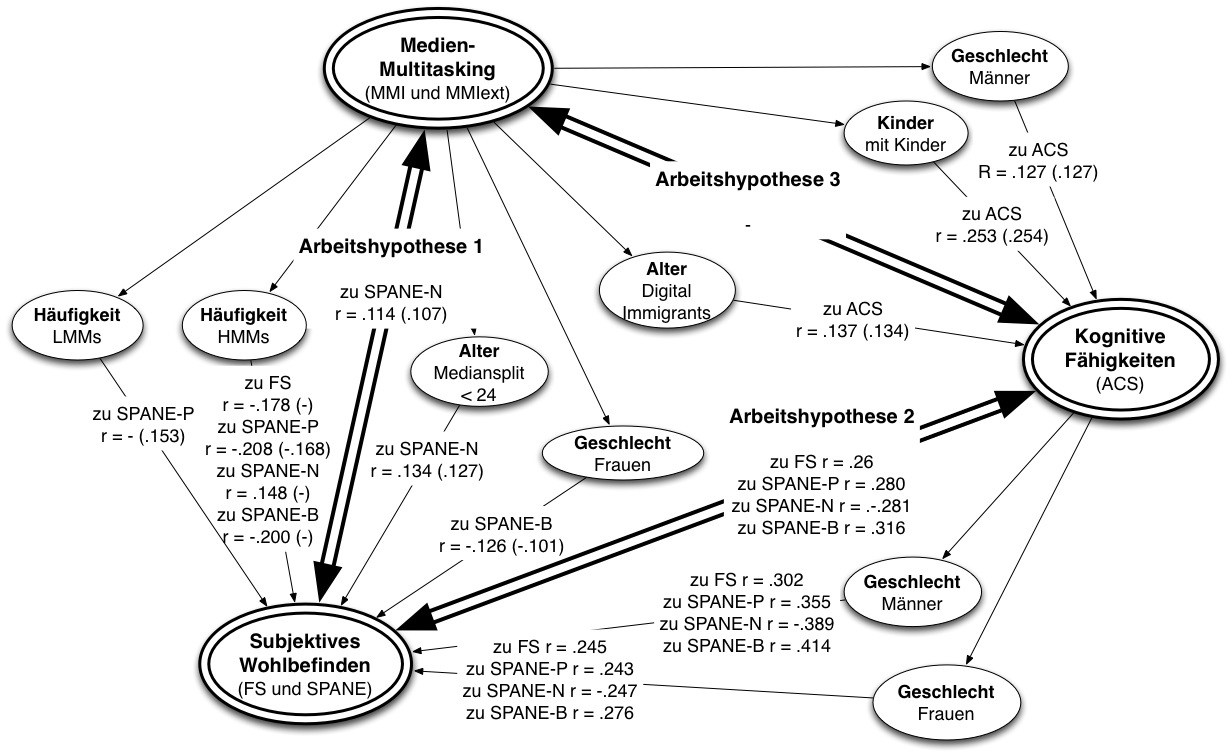
\includegraphics[scale=0.5, angle=90]{images/grafiken/Zusammenhang_Zusammenfassung_v2.jpg}
     \caption{Zusammenfassende Ergebnisse der Variablen gross}
     \label{pic.ergebniss.zusammenfassungGross}
\end{figure}

\end{RaggedRight}
